% uw-wkrpt-se.tex - An example work report that uses uw-wkrpt.cls
% Copyright (C) 2002,2003  Simon Law
% 
% This program is free software; you can redistribute it and/or modify
% it under the terms of the GNU General Public License as published by
% the Free Software Foundation; either version 2 of the License, or
% (at your option) any later version.
% 
% This program is distributed in the hope that it will be useful,
% but WITHOUT ANY WARRANTY; without even the implied warranty of
% MERCHANTABILITY or FITNESS FOR A PARTICULAR PURPOSE.  See the
% GNU General Public License for more details.
% 
% You should have received a copy of the GNU General Public License
% along with this program; if not, write to the Free Software
% Foundation, Inc., 59 Temple Place, Suite 330, Boston, MA  02111-1307  USA
%
%%%%%%%%%%%%%%%%%%%%%%%%%%%%%%%%%%%%%%%%%%%%%%%%%%%%%%%%%%%%%%%%%%%%%
%
% We begin by calling the workreport class which includes all the
% definitions for the macros we will use.
\documentclass[se,blockletter]{uw-wkrpt}

% LaTeX preamble: load some packages to add functionality
\usepackage{graphicx} % Include graphic importing

\usepackage[T1]{fontenc} % Better fonts
\usepackage{ae,aecompl}

\usepackage{indentfirst} % Indent first paragraph of each section

% Use biblatex for references
\usepackage[style=ieee,sorting=none,dateabbrev=false]{biblatex}
\bibliography{uw-wkrpt-bib}

% This needs to be the last package loaded
\usepackage[pdftex]{hyperref} % Generate PDF links and bookmarks.
\hypersetup{
  bookmarks=true,
  bookmarksnumbered=true
}

% Now we will begin writing the document.
\begin{document}

%%%%%%%%%%%%%%%%%%%%%%%%%%%%%%%%%%%%%%%%%%%%%%%%%%%%%%%%%%%%%%%%%%%%%
%% IMPORTANT INFORMATION
%%%%%%%%%%%%%%%%%%%%%%%%%%%%%%%%%%%%%%%%%%%%%%%%%%%%%%%%%%%%%%%%%%%%%

%% First we, should create a title page.  This is done below:
% Fill in the title of your report.
\title{Application of Machine Learning Models as a Solution to Hyperbola Identification in Ground Penetrating Radar Data}

% Fill in your name.
\author{Xiang Yi (Irene) Chen}

% Fill in your student ID number.
\uwid{20707344}

% Fill in your home address.
\address{277 Lester Street \\*
         Waterloo, ON\ \ N2L 3W6}

% Fill in your employer's name.
\employer{Sensors \& Software Inc.}

% Fill in your employer's city and province.
\employeraddress{Mississauga, ON}

% Fill in your school's name.
\school{University of Waterloo}

% Fill in your faculty name.
\faculty{Software Engineering}

% Fill in your student user ID
\userid{xy29chen}

% Fill in your e-mail address.
\email{irene.chen@edu.uwaterloo.ca}

% Fill in your term.
\term{1B}

% Fill in your program.
\program{Software Engineering}

% Fill in the department chair's name.
\chair{Dr.\ Derek\ Rayside}

% Fill in the department chair's mailing address.
\chairaddress{Software Engineering\\*
              University of Waterloo\\*
	      	 Waterloo, ON\ \ N2L 3G1}

% If you are writing an "SE-confidential" report, uncomment the next line.
%\confidential{SE-confidential}

% If you want to specify the date, fill it in here.  If you comment out
% this line, today's date will be substituted.
\date{August 21, 2018}

% Now, we ask LaTeX to generate the title.
\maketitle


\newcommand{\thecompany}{Sensors \& Software Inc.}

%%%%%%%%%%%%%%%%%%%%%%%%%%%%%%%%%%%%%%%%%%%%%%%%%%%%%%%%%%%%%%%%%%%%%
%% FRONT MATTER
%%%%%%%%%%%%%%%%%%%%%%%%%%%%%%%%%%%%%%%%%%%%%%%%%%%%%%%%%%%%%%%%%%%%%
%% \frontmatter will make the \section commands ignore their numbering,
%% it will also use roman page numbers.
\frontmatter

% After this, we must create a letter of submission.
\begin{letter}

The following work term report, entitled ``\thetitle'', has been prepared for \theemployer{} as my first work term report for my \theterm{} term. The objective of this work term report is to explore the feasibility of different machine learning models to the problem of hyperbola recognition and classification in ground penetrating radar data. 

I would like to thank my supervisor, Adam Fazzari for providing support and guidance along the way, as well as my co-workers for furthering my understanding of ground penetrating radars, from usage to data interpretation. Finally I would like to thank \theemployer{}, a major provider of ground penetrating radar systems, for creating this opportunity and setting me up with the dataset and other resources needed to retrain the models. 

\end{letter}

\section{Executive Summary}
The following report investigates the suitability of a small sample of pre-trained machine learning models, in response to the challenge of identifying hyperbolas in ground penetrating radar (GPR). The problem stems from the fact that hyperbola artefacts in GPR data are highly contextual, and present themselves in many different forms. As such, streamlining the interpretation process with software aids for GPR users proves itself to be a challenge due to the visual variety in GPR data.

However, the identification of hyperbola may be solved with the use of machine learning training. Hence, and exploration of convolutional neural networks (CNN), followed by a comparison of three notable CNN models---the Inception V3 model, as well as MobileNet V1 model, and VGG 19 model---to determine their suitability given restrictions to this identification problem. The choice of model was then tested and ultimately proven by a proof-of-concept application to hyperbola identification.

Based on limitations in labelled datasets, restricted training time as well as training environment, the decision to use MobileNet model was made based on the trade-off between model distributivity versus accuracy and training load, with a higher emphasis on its lightweight architecture. The final proof-of-concept model was able to achieve general hyperbola detection, of up to 13 detection per image. Its resulting classifier output was merely 22MB in size, trained by 171 labelled images for over 4000 steps.

Recommendations to TODO about the model's setup and training based on these limitations were made, in hopes to further improve the performance of the model. 

\subsection{Disclaimer}
The pre-trained models and their retraining modules are publicly available on GitHub. They've been applied with proprietary GPR data provided by \thecompany{}  

% Next, we need to make a Table of Contents, List of Figures and 
% List of Tables.  You will most likely need to run LaTeX twice to
% get these correct.  The first pass for LaTeX to figure out the
% labels, and the second pass to put in the right references.
\tableofcontents
\listoffigures
\listoftables

%%%%%%%%%%%%%%%%%%%%%%%%%%%%%%%%%%%%%%%%%%%%%%%%%%%%%%%%%%%%%%%%%%%%%
%% REPORT BODY
%%%%%%%%%%%%%%%%%%%%%%%%%%%%%%%%%%%%%%%%%%%%%%%%%%%%%%%%%%%%%%%%%%%%%
%% \main will make the \section commands numbered again,
%% it will also use arabic page numbers.
\mainmatter

% You must have an Introduction
\section{Introduction}\label{sec:intro}
Ground Penetrating Radar (GPR) solutions serve a wide range of uses, from underground utility locating, to pavement or ice thickness mapping, to forensics as well as archaeology. However, because of this varied usage---combined with pre-processing and post-processing---GPR data presents itself in many various ways. Hence, interpretation of GPR data is one of the most error-prone aspects of using GPR solutions.

\subsection{Problem Statement}
One of the biggest challenges of GPR data interpretation is to avoid false positives, such as extreme ringing caused by metal, 
as well as interference caused by rebounding air waves off the data collection site.

\thecompany{}'s software is able to apply velocity fitting and other transformations to GPR data to improve and simplify data interpretation, such as identifying false-positive air waves in GPR data through a calculation of its velocity. However, the first and most limiting step to this process is to allow the software to locate hyperbola---evidence of a disturbance in the soil caused by an object.

\subsection{Proposal of Solution}
Since machine learning has been making advances in the field of computer vision, it seems to be a fit tool to solve this bottleneck in this interpretation process.

Machine learning, in the broadest of terms, is a subset of computer science which allows programs to improve and "learn" without explicitly being told what exactly to do---the construction of algorithms to make predictions based on recognition of patterns on a data set and to make changes to itself so that its future performance is improved. 

Specifically, object detection and localization problems generally involve training feature extraction: associating certain characteristics of the image with different weights of importance based on their reoccurrence. In this problem, a hyperbola feature might consist of its curved nature. In this case, the presence---or lack thereof---of hyperbolas in GPR data will be explored with machine learning solutions, as well as their differentiation from other forms of features in GPR data, such as metal ringing and boundaries in the soil.

The follow section will be analysing the steps in a small sample of machine learning models, as well as the transferability and possibility of integration into existing GPR systems. The comparison process will be taking the following criteria into account:
\begin{itemize}
\item Correctness of learning, based on the core transformations of the architecture of the model
\item Ease of being transferred for real-time detection, based on the model's cost of memory and processing on ARM systems
\end{itemize} 

For the sake of quickly creating a proof-of-concept model, transfer learning will be applied to an existing open-source pre-trained model. Transfer learning entails modifying layers of existing mature models to customize the model while retaining its generic base layers. Specifically, the following pre-trained models will be explored, chosen for their current popularity and abundant availability in terms of support and resources: 
\begin{itemize}
\item Inception V3
\item MobileNet V2
\item VGG 19
\end{itemize}

% You must have either an Analysis or a Synthesis section.
\section{Comparison \& Analysis}
For the comparison of potential machine learning models, the general idea is to apply supervised learning, giving labelled datasets to distinguish hyperbolas in the image, then test the model with sets of unlabelled data of various degrees of resemblance to the training dataset.

\subsection{General Procedure}
\subsubsection{Retraining Neural Networks}
In the most intuitive sense, neural networks is an imitation of how the human brain works. Input features are weighted positively or negatively, forming and reinforcing connections between common features similar to neurons forming connections between each other.

Each layer performs a transformation on a single vector input, and the learning process is achieved by chaining these layers together, either cyclically or linearly. Deep learning refers to models with a great number of layers of transformations. The penultimate layer---the bottleneck---summarizes the extracted features, to allow the last layer to perform the classification task. 

Finally, weights of a model is a measure of the strength of the reinforcements between connections---equivalent to the output parameters to be learned throughout training. 

\subsubsection{Convolutional Neural Networks (CNN)}
Since for this hyperbola identification problem, GPR data can be easily converted to images, thus CNN will be used for their suitability with image inputs. A CNN is a subset of multi-layer neural networks, characterized by their convolution layer process---the union of integrals, or how much two functions overlap as one passes over the other---usually used for image classification. This overlap is the main idea behind how common features between images is reinforced and extracted. Processing is achieved by obtaining the union of the product of input images as matrices. \autocite[3]{cs231n_cnn}

The common components of CNN model architecture as as follows: the convolutional layer, the pooling layer, the ReLU activation layer and the fully-connected layer.

\begin{figure}
  \centering
  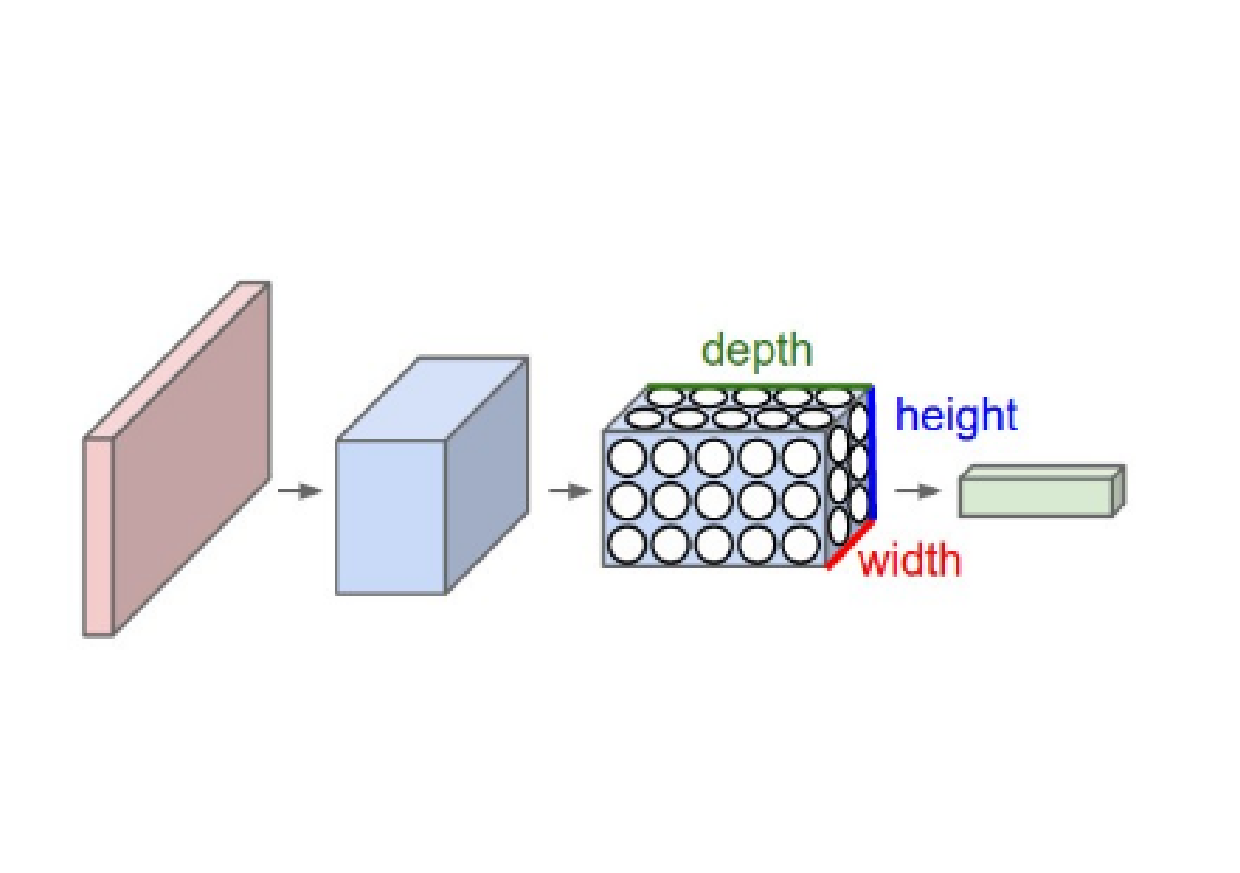
\includegraphics[height=6cm]{convolutional-neuron}
  \caption{A neuron in a convolutional network condensing image inputs into a 3D entity.~\cite{ref:}}
  \label{fig:cnn-neuron}
\end{figure}

Pooling is a transformation specific to convolutional neural networks: it combines clusters into a single entity to be used in the next layer, to condense and downsample previous operations with the intent to reduce parameters. This step assumes an image input and condenses the input into a 3-dimensional array, a convolutional neuron as seen in Figure~\ref{fig:cnn-neuron}. Max pooling, one of the most common types of pooling, is a downsampling function which takes the largest value from the prior cluster, effectively reducing the volume of data to process. Downsampling is not only used to reduce processing load, but by discarding select information, it prevents the model to be overfitted to the training dataset as in Figure~\ref{fig:overfitting}, hence less accurately solving the real-life problem. 

\begin{figure}
  \centering
  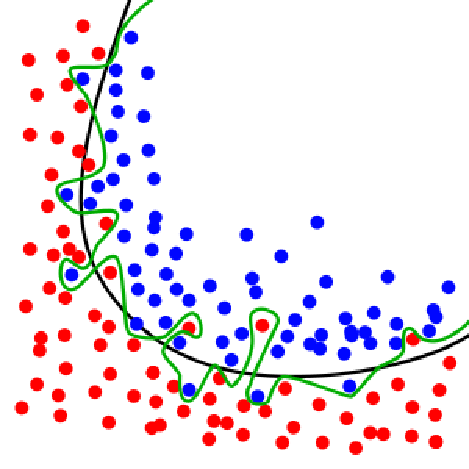
\includegraphics[height=4cm]{overfitting}
  \caption{Example overfitted model classifiying between two classes, a case to be avoided.~\cite{ref:}}
  \label{fig:overfitting}
\end{figure}

The convolution process is usually paired with a concatenation step as well as an activation ReLU layer. ReLU stands for rectified linear unit, a process to introduce non-linearity in the CNN, effectively performing $f(x) = max(0, x)$. This is a transformation on convolution outputs that doesn't affect the size of the matrix. 

Finally, the fully connected (FC) layer flattens the transformed image matrix. During this FC layer, the softmax function normalizes the output to be between 0 and 1, as a sigmoid function, similar to a categorical probability distribution. In this case, it should be executed in the end to bring the model closer to indicating the probability and likelihood of hyperbolas. 

\subsection{Inception V3}

Inception V3, also previously known as GoogleNet, is a CNN of five convolutional layers, along with the typical max pooling and softmax functions. However, it differs from the standard design of CNN models by its successive stacking scattered throughout the model between the convolutional layers, and is hence recognized as a deep training network.

\begin{figure}
  \centering
  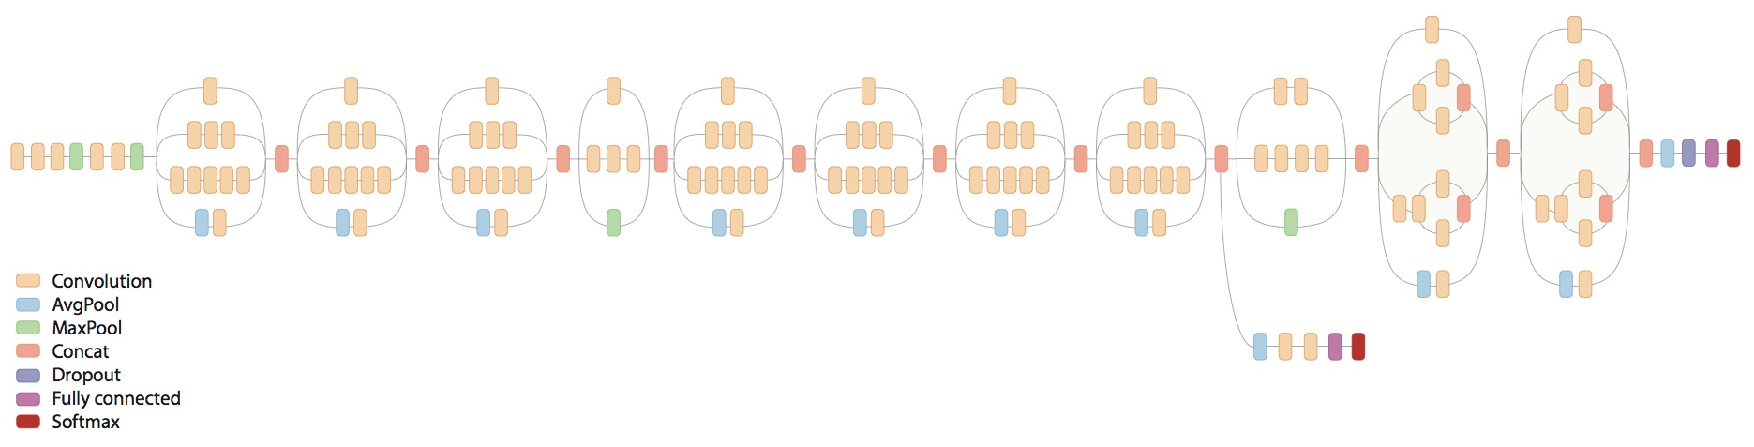
\includegraphics[height=11cm]{inception-architecture}
  \caption{Inception V3's CNN model architecture as described.~\cite{ref:}}
  \label{fig:inception-architecture}
\end{figure}

Simply, Inception extracts features at multiple levels, computing $1\times 1$, $3\times 3$, as well as $5 \times 5$ convolutional layers, which are concatenated afterwards as seen in Figure~\ref{fig:inception-architecture}. This particularity of the model allows the training to not only cover greater depths, but allows better receptive field variability of inputs, which in turn leads to being able to detect hyperbolas of different scales when applied. As well, the usage of smaller convolution layers stacked to replace a larger input through factorization, as demonstrated in Figure~\ref{fig:convolution-substitution}, also reduces the process load to train the model. This design is due to the fact that convolutions with larger spacial filters are disproportionally computationally-heavy. 

\begin{figure}
  \centering
  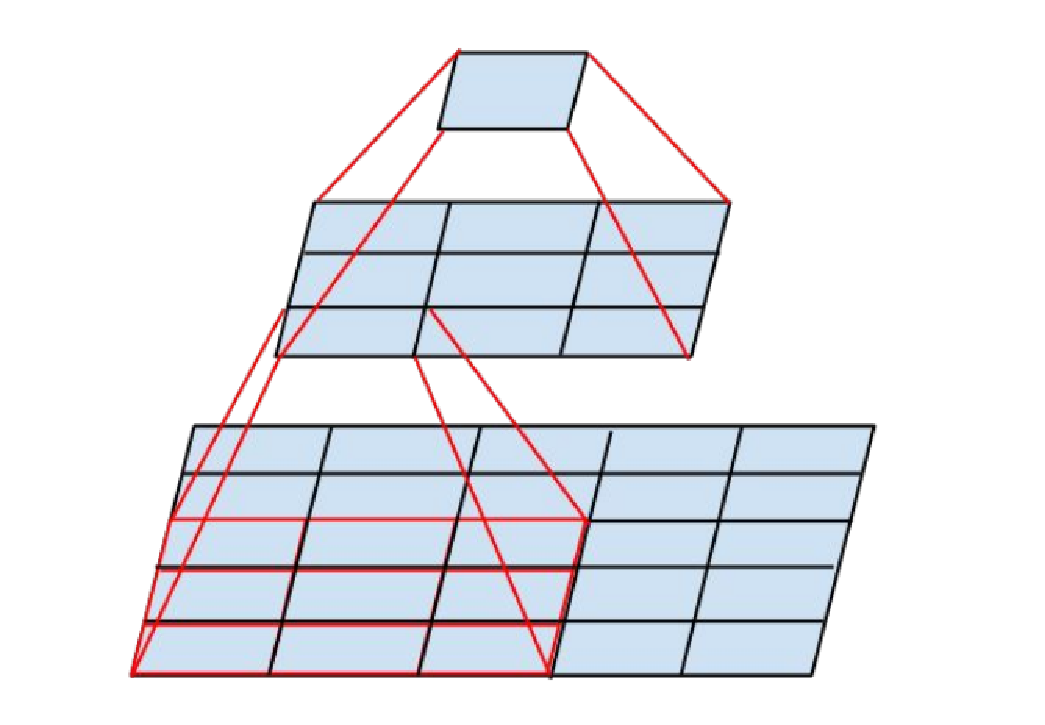
\includegraphics[height=5cm]{convolution-substitution}
  \caption{Factorizing and substituting convolution layers of smaller dimensions to cover the input matric.~\cite{ref:}}
  \label{fig:convolution-substitution}
\end{figure}

Although Inception's multi-layer convolution process is extremely desirable, by increasing the density of data of this model, it drastically increases the computational costs. Large $5\times 5$ convolutional operations are exponentially more expensive to compute, compared to their $3\times 3$ and $1\times 1$ counterparts.


Unlike many CNN models, Inception skips intermediary activation layers, making its computational cost much lower than the other two models compared. This makes Inception a likely candidate to train our hyperbola classifier problem in an environment where memory and computational capacity of the hardware is limited.

As for the result of the model, the weights for Inception V3 are small, coming in at 92MB, with a total depth of 159 stacked layers per training iteration. 

\subsection{MobileNet V1}
MobileNet, as its name suggests, is a CNN model specifically tailored to run on resource constrained environment such as mobile platforms. 

To lighten the processing, it applies a depth-wise separable process of convolutions similar to Inception (Figure ~\ref{fig:depthwise-separable-conv}). Essentially, a $3 \times 13$ factorized convolutional layer is applied to the input matrix linearly in the depth direction, then a $1 \times 1$ convolution concatenates the matrix back layer-wise called a point-wise convolution layer. MobileNet processes a total of 14 batches of convolution throughout the model, followed by one average pooling function as well as one fully connected layer, ending with the typical softmax function.

\begin{figure}
  \centering
  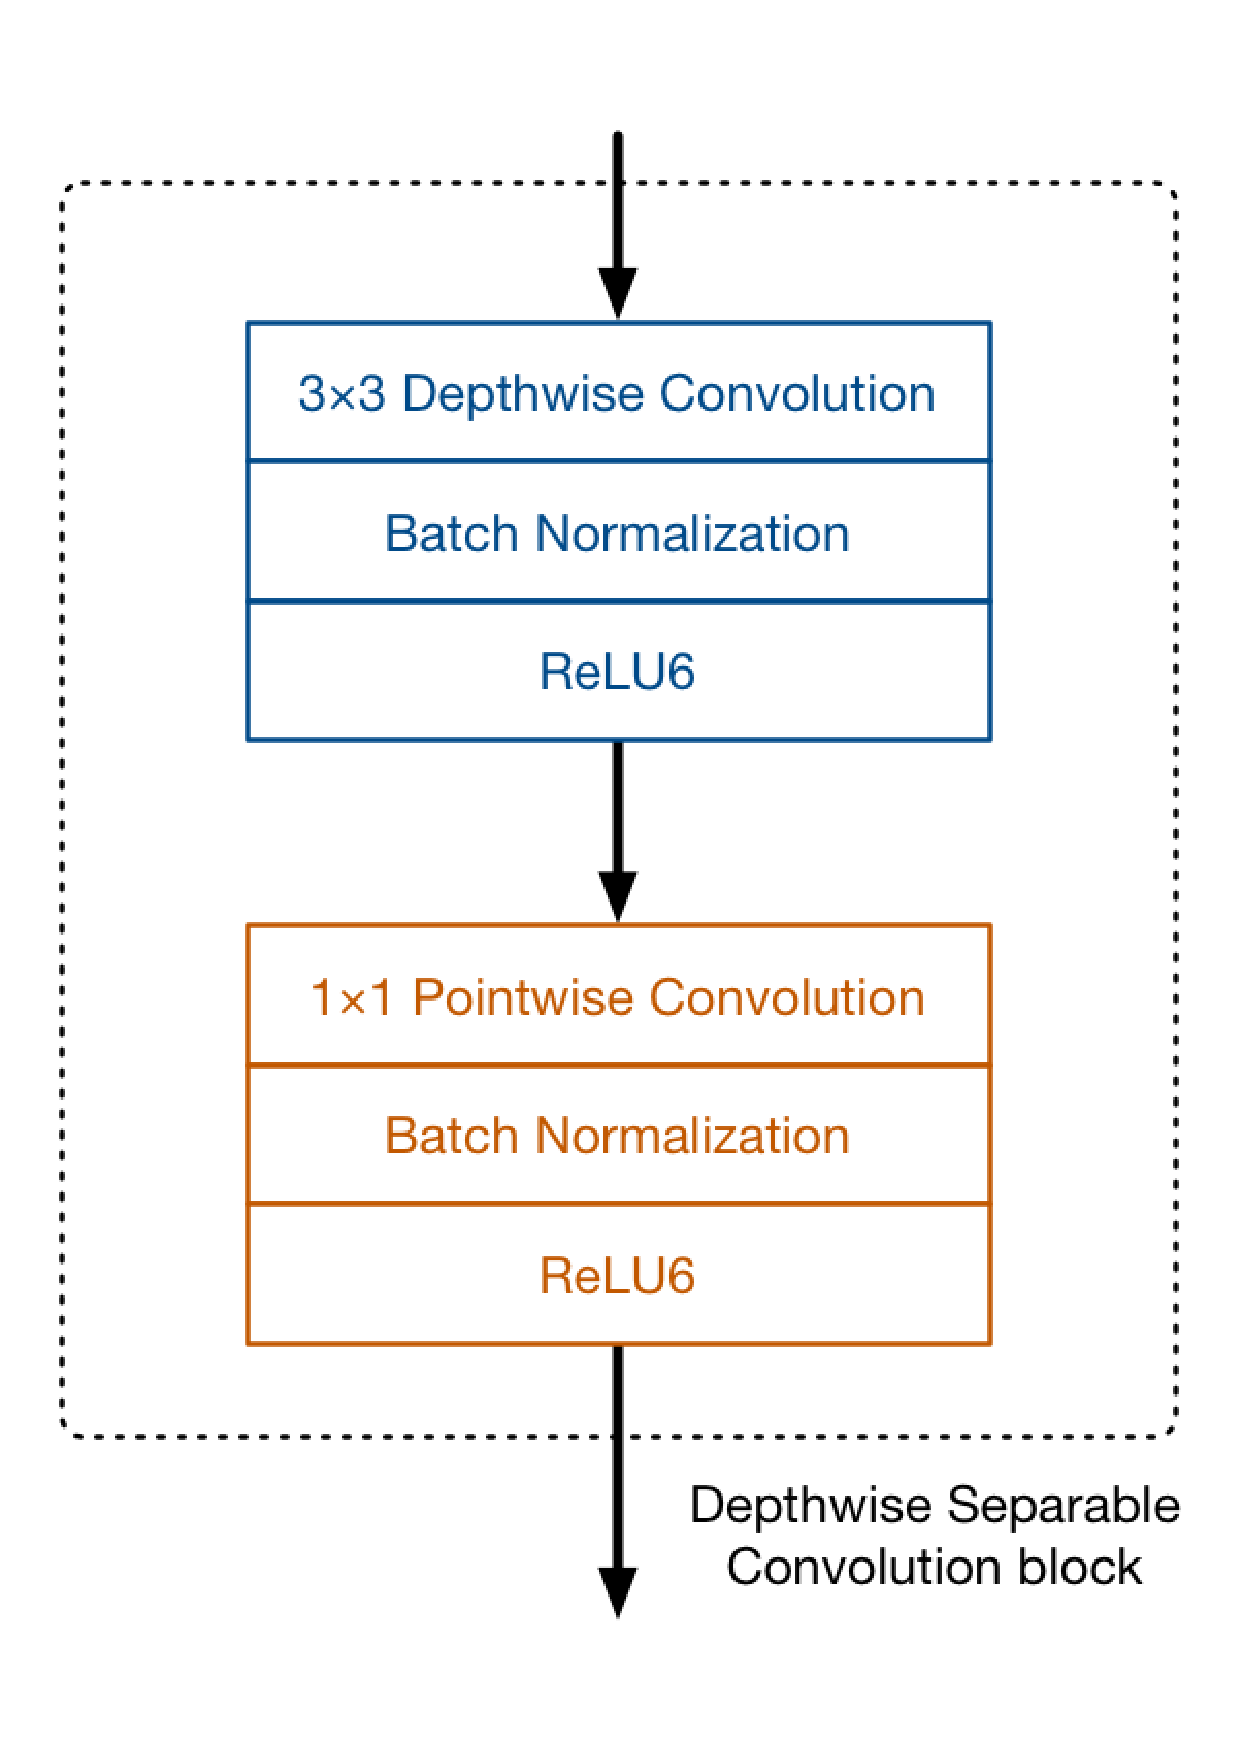
\includegraphics[height=4cm]{depthwise-separable-conv}
  \caption{Visualizing the depth-wise separable convolution process.~\cite{ref:}}
  \label{fig:depthwise-separable-conv}
\end{figure}

However, there is a trade-off in accuracy for this lightweight model. Using standards of ImageNet, in a comparison paper of these three models, MobileNet ranks on the lower end of the three models, achieving a Top-1 accuracy of 71.0---noticeably lower than both Inception V3 and VGG 19, as seen in Table \ref{tbl:top-1-comparison}

\begin{table}
\centering
 \begin{tabular}{|| c c ||} 
 \hline
 Model & Top-1 \\ [0.5ex] 
 \hline\hline
  Inception V3  & 78.0 \\
 \hline
  VGG 19  & 77.3  \\ 
 \hline
  MobileNet V1  & 71.0 \\ [1ex] 
 \hline
\end{tabular}
\caption{ImageNet standards top-1 accuracy comparison between models.}
\label{tbl:top-1-comparison}
\end{table}

However, since the size of weights of the model, an expected 22MB, i

\subsection{VGG 19}
VGG 19 consists of five convolutional layers as well, $3 \times 3$ stacked on top of each other in increasing depth, designed by the Visual Geometry Group of Oxford. "19" stand for the number of weight layers in the network, the sum of five batches of convolutional layers as well as max pooling to reduce volume size and finally ending with two fully connected layers as well as a softmax process.

VGG's $3 \times 3$ convolutional layers amount to fixed reception fields. Hence, the model is limited to an optimal size of hyperbola to be detected, resulting to over-fitting the model to a certain type of expected GPR data input.  

\begin{figure}
  \centering
  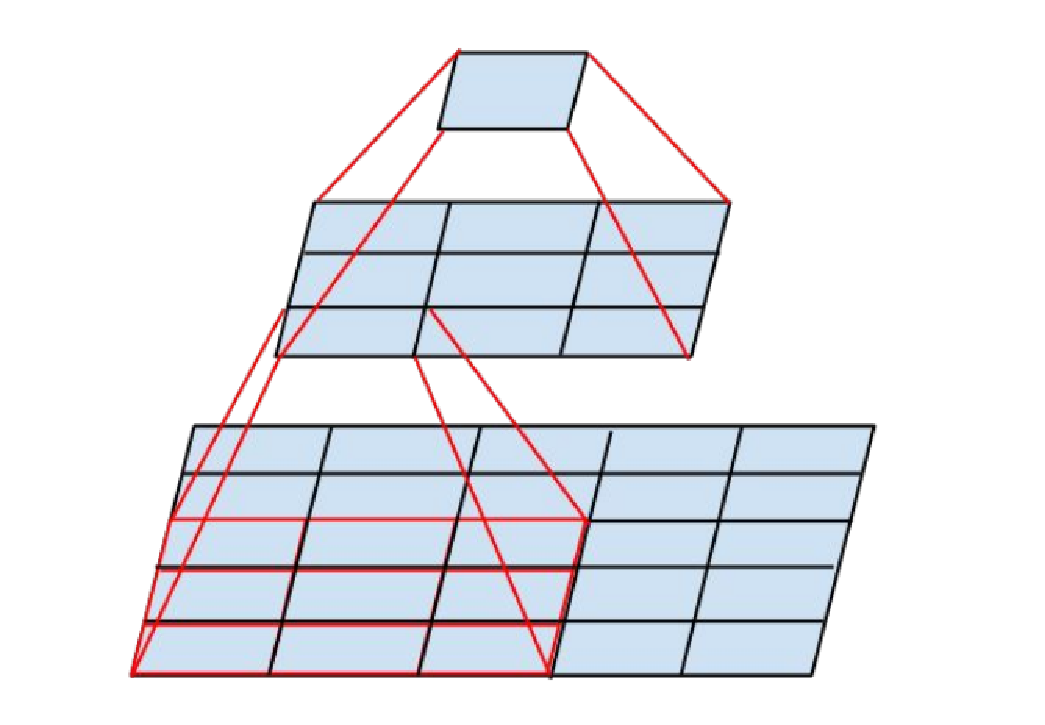
\includegraphics[height=5cm]{convolution-substitution}
  \caption{Factorizing and substituting convolution layers of smaller dimensions to cover the input matric.~\cite{ref:}}
  \label{fig:convolution-substitution}
\end{figure}

Based on the older AlexNet model---which is characterized by implementing a dropout function after each FC layer---the VGG model attempts to compensate for overfitting with a dropout process after each fully connected layer. Figure ~\ref{fig:VGG-vs-AlexNet}
shows the advantageous architecture of VGG.

\begin{figure}
  \centering
  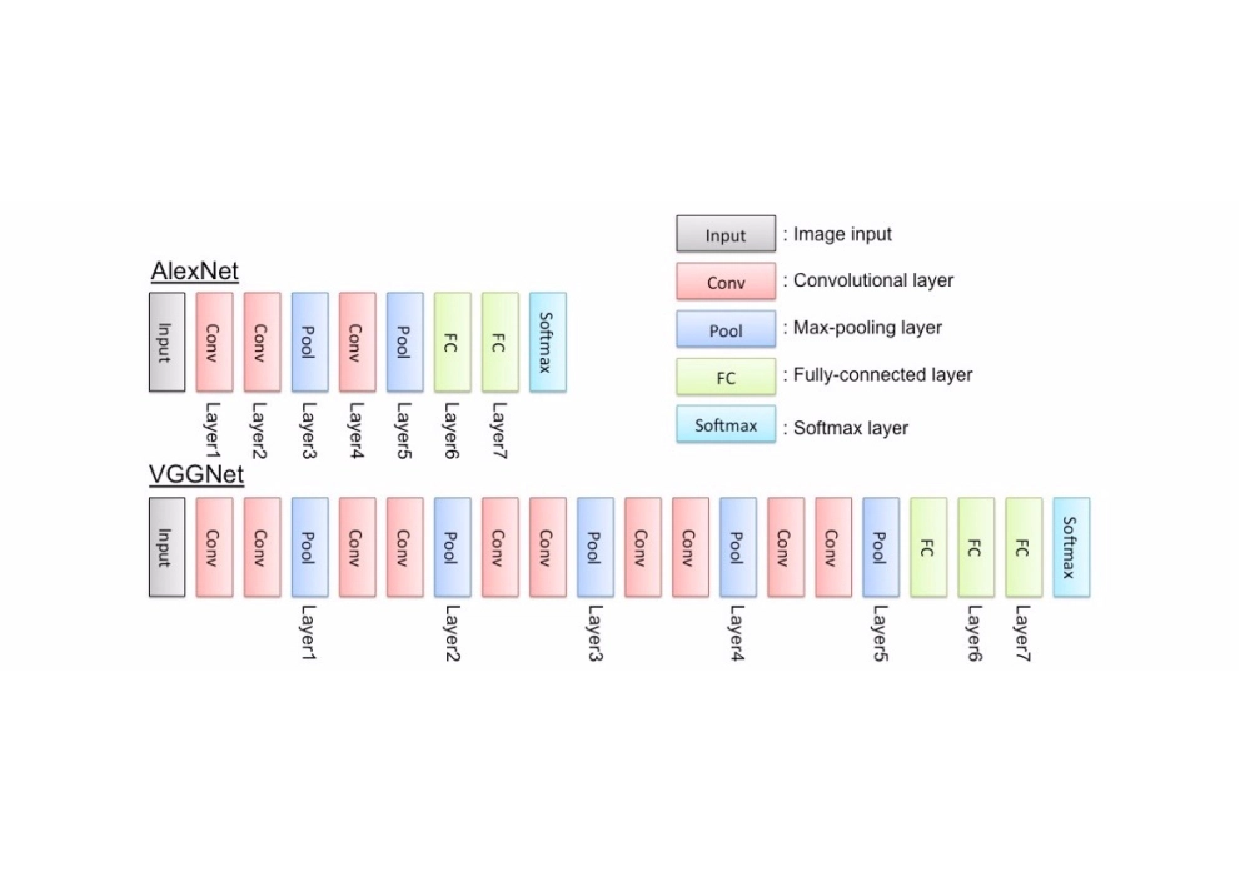
\includegraphics[height=8cm]{VGG-vs-AlexNet}
  \caption{A comparison of VGG's model structure, ~\cite{ref:}}
  \label{fig:VGG-vs-AlexNet}
\end{figure}

However, the downside of this phenomenal accuracy is in its difficult deployment and training process due to the great calculation requirements---a disadvantage both in processing speed and memory requirements. 

The network architecture weights themselves are quite large. Due to its depth and number of fully-connected nodes, the VGG model itself is over 574MB for VGG19. Hence, the biggest drawbacks of VGG, despite its good depth and accuracy, would be hard to deploy onto \thecompany{}'s GPR systems, and would only be something usable in EKKO Project, a post-processing software product. Due to this great drawback, the trade-off for accuracy of the VGG19 model is deemed too large and expensive to be used in this hyperbola classification situation.


\section{Results}

Through the proof-of-concept classifier, experimental results show that MobileNet is about 3 times as fast as Inception and 10 times as fast as VGG, running at an average of 26 seconds per batch of 24 images. Despite slightly lower accuracy, it still performed reasonably accurate, with over 4000 steps of training using a pre-processed labelled dataset of 171 images. 

\begin{figure}
  \centering
  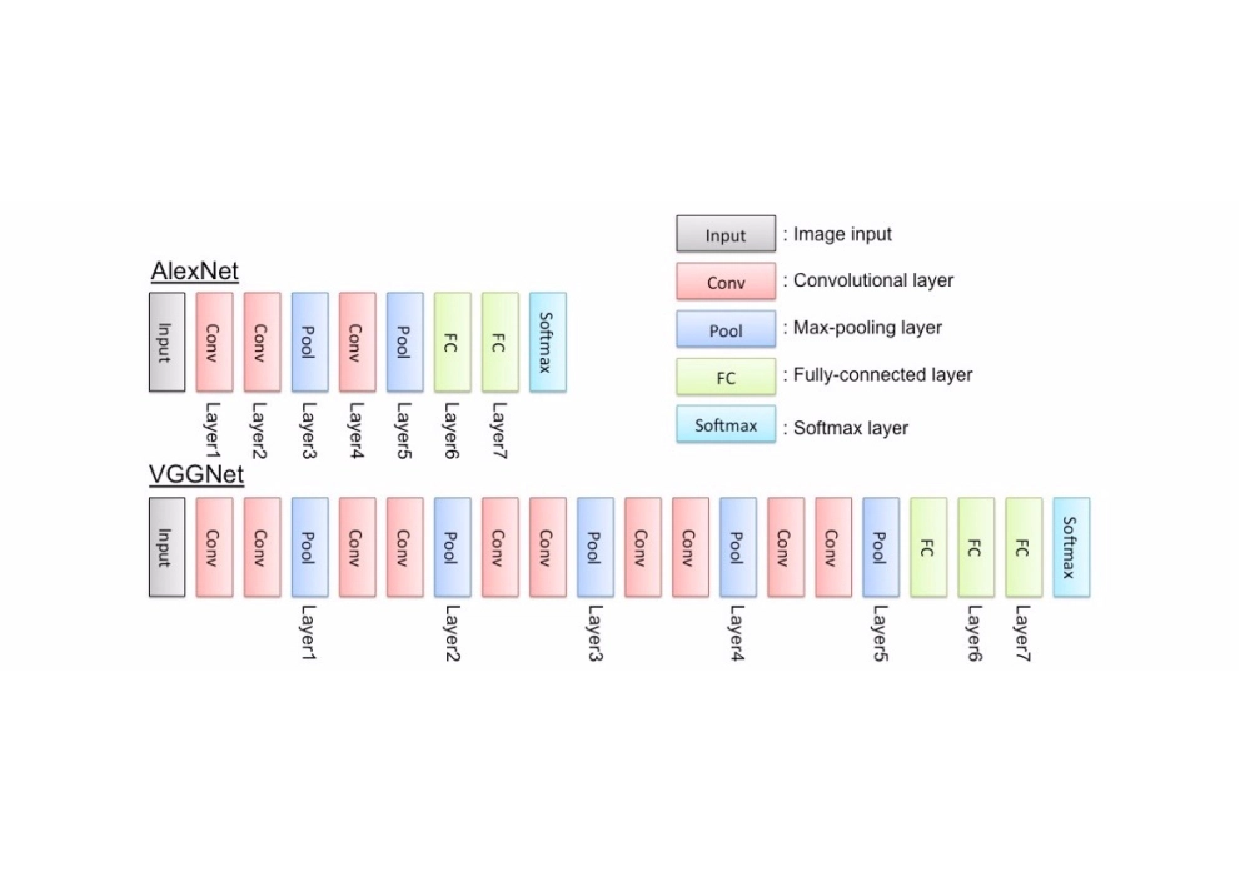
\includegraphics[height=8cm]{VGG-vs-AlexNet}
  \caption{~\cite{ref:}}
  \label{fig:VGG-vs-AlexNet}
\end{figure}


\section{Conclusions}


\section{Recommendations}
My proof-of-concept consists of three training iterations


However, this is but a limited comparison of a small selection of models---though three very successful models. 


As well, needless to say, 
hyperbola detection and identification has proven itself to be a problem difficult to tailor to 


at this stage, the current proof-of-concept was trained within a manually created dataset, which is only a rough representation of hyperbola identification. To attempt to capture the full complexity of the problem, a better breadth of images---a wide variety of hyperbolas in different environments, different soil calibrations, different collection speeds and GPR stacking---is required to avoid the model to over-fit to noisy or coincidental features in the GPR data.


No thorough understanding of the complexity of these machine learning models, which is a challenge to adapt and make changes to the CNN.
If scaled or applied to the problem naively, certain computational gains during training can be lost, which immediately voids its advantage over other models. 

%%%%%%%%%%%%%%%%%%%%%%%%%%%%%%%%%%%%%%%%%%%%%%%%%%%%%%%%%%%%%%%%%%%%%
%% BACK MATTER
%%%%%%%%%%%%%%%%%%%%%%%%%%%%%%%%%%%%%%%%%%%%%%%%%%%%%%%%%%%%%%%%%%%%%
%% \backmatter will make the \section commands ignore their numbering,
\backmatter

% Here, we insert a References section, which will be formatted properly.
% The list of works you have referenced should be specified in the preamble.
% In this template, the file is uw-wkrpt-bib.bib.
%
% Note, you will need to process the document in a certain order.  First,
% run LaTeX.  The % first pass will allow LaTeX to build a list of 
% references, it may % emit warning messages such as:
%   LaTeX Warning: Reference `app:gnugpl' on page 4 undefined on input line 277.
%   LaTeX Warning: There were undefined references.
% This is normal.  Now you run BiBTeX in order to generate the proper
% layout for the references.  After this, you run LaTeX once more.

\printbibliography[heading=bibintoc]


%%%%%%%%%%%%%%%%%%%%%%%%%%%%%%%%%%%%%%%%%%%%%%%%%%%%%%%%%%%%%%%%%%%%%
%% APPENDICES
%%%%%%%%%%%%%%%%%%%%%%%%%%%%%%%%%%%%%%%%%%%%%%%%%%%%%%%%%%%%%%%%%%%%%
%% \appendix will reset \section numbers and turn them into letters.
%%
%% Don't forget to refer to all your appendices in the main report.
\appendix


\end{document}
